\documentclass[10pt,fleqn]{article} % Default font size and left-justified equations
\usepackage[%
    pdftitle={Modélisation systèmes multiphysiques : Modélisation linéaire et non linéaire},
    pdfauthor={Xavier Pessoles}]{hyperref}
    
\usepackage{listingsutf8}


%%%%%%%%%%%%%%%%%%%%%%%%%%%%%%%%%%%%%%%%%
% Original author:
% Mathias Legrand (legrand.mathias@gmail.com) with modifications by:
% Vel (vel@latextemplates.com)
% License:
% CC BY-NC-SA 3.0 (http://creativecommons.org/licenses/by-nc-sa/3.0/)
%%%%%%%%%%%%%%%%%%%%%%%%%%%%%%%%%%%%%%%%%

%----------------------------------------------------------------------------------------
%	VARIOUS REQUIRED PACKAGES AND CONFIGURATIONS
%----------------------------------------------------------------------------------------

%\usepackage[top=2.5cm,bottom=2cm,left=2cm,right=2cm,headsep=40pt,a4paper]{geometry} % Page margins
\usepackage[top=2cm,bottom=2cm,left=2cm,right=2cm,a4paper]{geometry} % Page margins

\usepackage{graphicx} % Required for including pictures

\usepackage{lipsum} % Inserts dummy text

\usepackage{tikz} % Required for drawing custom shapes

\usepackage[francais]{babel} % English language/hyphenation
\frenchbsetup{StandardLists=true} % Pour éviter la collision babel enumitem pour les listes

\usepackage{enumitem} % Customize lists
\setlist{nolistsep} % Reduce spacing between bullet points and numbered lists

\usepackage{booktabs} % Required for nicer horizontal rules in tables

\usepackage{xcolor} % Required for specifying colors by name
%\definecolor{ocre}{RGB}{243,102,25} % Define the orange color used for highlighting throughout the book
 \definecolor{ocre}{RGB}{49,133,156} % Couleur ''bleue''
\definecolor{violetf}{RGB}{112,48,160} % Couleur ''violet''
\usepackage{enumitem}
\usepackage{pifont} % Pour les dinglist
\usepackage{multicol}
\usepackage{array} % Centrage vertical dans les tableaux
\usepackage{schemabloc}

%----------------------------------------------------------------------------------------
%	FONTS
%----------------------------------------------------------------------------------------
\usepackage{bm}
\usepackage{multicol}
\usepackage{siunitx}
\sisetup{output-decimal-marker = {,}}


\usepackage{avant} % Use the Avantgarde font for headings
%\usepackage{times} % Use the Times font for headings
%\usepackage{mathptmx} % Use the Adobe Times Roman as the default text font together with math symbols from the Sym­bol, Chancery and Com­puter Modern fonts
\usepackage[adobe-utopia]{mathdesign}
\usepackage{microtype} % Slightly tweak font spacing for aesthetics
\usepackage[utf8]{inputenc} % Required for including letters with accents
\usepackage[T1]{fontenc} % Use 8-bit encoding that has 256 glyphs

%----------------------------------------------------------------------------------------
%	Code PYTHON
%----------------------------------------------------------------------------------------

\usepackage[rerun=errors,makestderr=true]{pythontex}
\usepackage{listings}
\lstloadlanguages{Python}

\lstset{language=Python,
        columns=fullflexible,
%	  identifierstyle=\sffamily,
	  basicstyle=\ttfamily,
	  keywordstyle=\bf,
	  commentstyle=\normalfont,
%	  numbers=none, numberstyle=\small, numbersep=30pt, %gestion numérotation
%	  showstringspaces=false,%pour cacher le symbole d'espacement dans les chaînes
	  breaklines=true, %passage à la ligne automatique
	  prebreak=\mbox{$\swarrow$},
%	  includerangemarker=false, % pour inclure partiellement des fichiers
%	  rangeprefix=\#\ 
	  }


\lstset{
  literate={ö}{{\"o}}1
           {ä}{{\"a}}1
           {ü}{{\"u}}1
           {é}{{\'e}}1
           {è}{{\`e}}1
           {ê}{{\^e}}1
           {à}{{\`a}}1
           {â}{{\^a}}1
           {ù}{{\`u}}1
           {ç}{{\c{c}}}1
           {î}{{\^{i}}}1
           {ô}{{\^{o}}}1
           {É}{{\'{E}}}1
}


%----------------------------------------------------------------------------------------
%	BIBLIOGRAPHY AND INDEX
%----------------------------------------------------------------------------------------

%\usepackage[style=alphabetic,citestyle=numeric,sorting=nyt,sortcites=true,autopunct=true,babel=hyphen,hyperref=true,abbreviate=false,backref=true,backend=biber]{biblatex}
\usepackage[style=alphabetic,citestyle=numeric,sorting=nyt,sortcites=true,autopunct=true,hyperref=true,abbreviate=false,backref=true,backend=biber]{biblatex}
\addbibresource{bibliography.bib} % BibTeX bibliography file
\defbibheading{bibempty}{}

\usepackage{calc} % For simpler calculation - used for spacing the index letter headings correctly
\usepackage{makeidx} % Required to make an index
\makeindex % Tells LaTeX to create the files required for indexing

%----------------------------------------------------------------------------------------
%	MAIN TABLE OF CONTENTS
%----------------------------------------------------------------------------------------

\usepackage{titletoc} % Required for manipulating the table of contents

\setcounter{tocdepth}{2}     % Dans la table des matieres
\setcounter{secnumdepth}{2}

\contentsmargin{0cm} % Removes the default margin

% Part text styling
\titlecontents{part}[0cm]
{\addvspace{20pt}\centering\large\bfseries}
{}
{}
{}

% Chapter text styling
\titlecontents{chapter}[1.25cm] % Indentation
{\addvspace{12pt}\large\sffamily\bfseries} % Spacing and font options for chapters
{\color{ocre!60}\contentslabel[\Large\thecontentslabel]{1.25cm}\color{ocre}} % Chapter number
{\color{ocre}}  
{\color{ocre!60}\normalsize\;\titlerule*[.5pc]{.}\;\thecontentspage} % Page number

% Section text styling
\titlecontents{section}[1.25cm] % Indentation
{\addvspace{3pt}\sffamily\bfseries} % Spacing and font options for sections
{\color{ocre!60}\contentslabel[\thecontentslabel]{1.25cm} \color{ocre}} % Section number
{\color{ocre}}
{\hfill\color{ocre!60}\thecontentspage} % Page number
[]

% Subsection text styling
\titlecontents{subsection}[1.25cm] % Indentation
{\addvspace{1pt}\sffamily\small} % Spacing and font options for subsections
{\contentslabel[\thecontentslabel]{1.25cm}} % Subsection number
{}
{\ \titlerule*[.5pc]{.}\;\thecontentspage} % Page number
[]


% Subsection text styling
\titlecontents{subsubsection}[1.25cm] % Indentation
{\addvspace{1pt}\sffamily\small} % Spacing and font options for subsections
{\contentslabel[\thecontentslabel]{1.25cm}} % Subsection number
{}
{\ \titlerule*[.5pc]{.}\;\thecontentspage} % Page number
[]

% List of figures
\titlecontents{figure}[0em]
{\addvspace{-5pt}\sffamily}
{\thecontentslabel\hspace*{1em}}
{}
{\ \titlerule*[.5pc]{.}\;\thecontentspage}
[]

% List of tables
\titlecontents{table}[0em]
{\addvspace{-5pt}\sffamily}
{\thecontentslabel\hspace*{1em}}
{}
{\ \titlerule*[.5pc]{.}\;\thecontentspage}
[]

%----------------------------------------------------------------------------------------
%	MINI TABLE OF CONTENTS IN PART HEADS
%----------------------------------------------------------------------------------------

% Chapter text styling
\titlecontents{lchapter}[0em] % Indenting
{\addvspace{15pt}\large\sffamily\bfseries} % Spacing and font options for chapters
{\color{ocre}\contentslabel[\Large\thecontentslabel]{1.25cm}\color{ocre}} % Chapter number
{}  
{\color{ocre}\normalsize\sffamily\bfseries\;\titlerule*[.5pc]{.}\;\thecontentspage} % Page number

% Section text styling
\titlecontents{lsection}[0em] % Indenting
{\sffamily\small} % Spacing and font options for sections
{\contentslabel[\thecontentslabel]{1.25cm}} % Section number
{}
{}

% Subsection text styling
\titlecontents{lsubsection}[.5em] % Indentation
{\normalfont\footnotesize\sffamily} % Font settings
{}
{}
{}

%----------------------------------------------------------------------------------------
%	PAGE HEADERS
%----------------------------------------------------------------------------------------

\usepackage{fancyhdr} % Required for header and footer configuration



\pagestyle{fancy}
 \renewcommand{\headrulewidth}{0pt}
 \fancyhead{}
 
 % ENTETES de page
 \fancyhead[L]{%
 \begin{tikzpicture}[overlay]
\node(logo) at (1,0)
    {
\includegraphics[width=2cm]{logo_lycee.png}};
\end{tikzpicture}
 %\noindent\begin{minipage}[c]{2.6cm}%
 %
\includegraphics[width=2cm]{logo_lycee.png}%
 %\end{minipage}
}

\fancyhead[C]{\rule{8cm}{.5pt}}

 \fancyhead[R]{%
 \noindent\begin{minipage}[c]{3cm}
 \begin{flushright}
 \footnotesize{\textit{\textsf{\xxtete}}}%
 \end{flushright}
 \end{minipage}
}

 \fancyfoot{}
 % PIEDS de page
\fancyfoot[C]{\rule{12cm}{.5pt}}
\renewcommand{\footrulewidth}{0.2pt}
\fancyfoot[C]{\footnotesize{\bfseries \thepage}}
\fancyfoot[L]{ 
\begin{minipage}[c]{.4\linewidth}
\noindent\footnotesize{{\xxauteur}}
\end{minipage}}

\fancyfoot[R]{\footnotesize{\xxpied}
\ifthenelse{\isodd{\value{page}}}{
\begin{tikzpicture}[overlay]
\node[shape=rectangle, 
      rounded corners = .25 cm,
	  draw= ocre,
	  line width=2pt, 
	  fill = ocre!10,
	  minimum width  = 2.5cm,
	  minimum height = 3cm,] at (\xxposongletx,\xxposonglety) {};
\node at (\xxposonglettext,\xxposonglety) {\rotatebox{90}{\textbf{\large\color{ocre}{\xxonglet}}}};
%{};
\end{tikzpicture}}{}
}



%
%
%
% Removes the header from odd empty pages at the end of chapters
\makeatletter
%\renewcommand{\cleardoublepage}{
%\clearpage\ifodd\c@page\else
%\hbox{}
%\vspace*{\fill}
%\thispagestyle{empty}
%\newpage
%\fi}

%\fancypagestyle{plain}{%
%\fancyhf{} % vide l’en-tête et le pied~de~page.
%%\fancyfoot[C]{\bfseries \thepage} % numéro de la page en cours en gras
%% et centré en pied~de~page.
%\fancyfoot[R]{\footnotesize{\xxpied}}
%\fancyfoot[C]{\rule{12cm}{.5pt}}
%\renewcommand{\footrulewidth}{0.2pt}
%\fancyfoot[C]{\footnotesize{\bfseries \thepage}}
%\fancyfoot[L]{ 
%\begin{minipage}[c]{.4\linewidth}
%\noindent\footnotesize{{\xxauteur}}
%\end{minipage}}}

\fancypagestyle{plain}{%
\fancyhf{} % vide l’en-tête et le pied~de~page.
\fancyfoot[C]{\rule{12cm}{.5pt}}
\renewcommand{\footrulewidth}{0.2pt}
\fancyfoot[C]{\footnotesize{\bfseries \thepage}}
\fancyfoot[L]{ 
\begin{minipage}[c]{.4\linewidth}
\noindent\footnotesize{{\xxauteur}}
\end{minipage}}
\fancyfoot[R]{\footnotesize{\xxpied}}
}




%----------------------------------------------------------------------------------------
%	THEOREM STYLES
%----------------------------------------------------------------------------------------

% Conflit avec la police adobe
%\usepackage{amsmath,amsfonts,amssymb,amsthm} % For math equations, theorems, symbols, etc
\usepackage{amsmath,amsthm}

\newcommand{\intoo}[2]{\mathopen{]}#1\,;#2\mathclose{[}}
\newcommand{\ud}{\mathop{\mathrm{{}d}}\mathopen{}}
\newcommand{\intff}[2]{\mathopen{[}#1\,;#2\mathclose{]}}
%\newtheorem{notation}{Notation}[chapter]
\newtheorem{notation}{Notation}[section]

% Boxed/framed environments
\newtheoremstyle{ocrenumbox}% % Theorem style name
{0pt}% Space above
{0pt}% Space below
{\normalfont}% % Body font
{}% Indent amount
{\small\bf\sffamily\color{ocre}}% % Theorem head font
{\;}% Punctuation after theorem head
{0.25em}% Space after theorem head
{\small\sffamily\color{ocre}\thmname{#1}\nobreakspace\thmnumber%{\@ifnotempty{#1}{}\@upn{#2}}% Theorem text (e.g. Theorem 2.1)
\thmnote{\nobreakspace\the\thm@notefont\sffamily\bfseries\color{black}---\nobreakspace#3.}} % Optional theorem note
\renewcommand{\qedsymbol}{$\blacksquare$}% Optional qed square


% Boite pour les corriges
\newtheoremstyle{correctionbox}% % Theorem style name
{0pt}% Space above
{0pt}% Space below
{\normalfont}% % Body font
{}% Indent amount
{\small\bf\sffamily\color{violet}}% % Theorem head font
{\;}% Punctuation after theorem head
{0.25em}% Space after theorem head
{\small\sffamily\color{ocre}\thmname{#1}\nobreakspace\thmnumber%{\@ifnotempty{#1}{}\@upn{#2}}% Theorem text (e.g. Theorem 2.1)
\thmnote{\nobreakspace\the\thm@notefont\sffamily\bfseries\color{black}---\nobreakspace#3.}} % Optional theorem note
\renewcommand{\qedsymbol}{$\blacksquare$}% Optional qed square



\newtheoremstyle{blacknumex}% Theorem style name
{5pt}% Space above
{5pt}% Space below
{\normalfont}% Body font
{} % Indent amount
{\small\bf\sffamily}% Theorem head font
{\;}% Punctuation after theorem head
{0.25em}% Space after theorem head
{\small\sffamily{\tiny\ensuremath{\blacksquare}}\nobreakspace\thmname{#1}\nobreakspace\thmnumber%{\@ifnotempty{#1}{}\@upn{#2}}% Theorem text (e.g. Theorem 2.1)
\thmnote{\nobreakspace\the\thm@notefont\sffamily\bfseries---\nobreakspace#3.}}% Optional theorem note

\newtheoremstyle{blacknumbox} % Theorem style name
{0pt}% Space above
{0pt}% Space below
{\normalfont}% Body font
{}% Indent amount
{\small\bf\sffamily}% Theorem head font
{\;}% Punctuation after theorem head
{0.25em}% Space after theorem head
{\small\sffamily\thmname{#1}\nobreakspace 
\thmnote{\nobreakspace\the\thm@notefont\sffamily\bfseries---\nobreakspace#3.}}% Optional theorem note

% Non-boxed/non-framed environments
\newtheoremstyle{ocrenum}% % Theorem style name
{5pt}% Space above
{5pt}% Space below
{\normalfont}% % Body font
{}% Indent amount
{\small\bf\sffamily\color{ocre}}% % Theorem head font
{\;}% Punctuation after theorem head
{0.25em}% Space after theorem head
{\small\sffamily\color{ocre}\thmname{#1}\nobreakspace%\thmnumber{\@ifnotempty{#1}{}\@upn{#2}}% Theorem text (e.g. Theorem 2.1)
\thmnote{\nobreakspace\the\thm@notefont\sffamily\bfseries\color{black}---\nobreakspace#3.}} % Optional theorem note
\renewcommand{\qedsymbol}{$\blacksquare$}% Optional qed square
\makeatother

% Environnement pour les titres de parties
\newtheoremstyle{partiebox} 
{0pt}% Space above
{0pt}% Space below
{\normalfont}% Body font
{}% Indent amount
{\small\bf\sffamily}% Theorem head font
{\;}% Punctuation after theorem head
{0.25em}% Space after theorem head




% Defines the theorem text style for each type of theorem to one of the three styles above
\newcounter{dummy} 
\numberwithin{dummy}{section}
\theoremstyle{ocrenumbox}
%\newtheorem{theoremeT}[dummy]{Théorème}
\newtheorem{theoremeT}[dummy]{Théorème}
\newtheorem{resultatT}[dummy]{Résultat}
\newtheorem{savoirT}[dummy]{Savoir}
\newtheorem{methodeT}[dummy]{Méthode}
\newtheorem{objectifT}[dummy]{Objectif}
%\newtheorem{problem}{Problem}[chapter]
\newtheorem{problem}{Problem}[section]
%\newtheorem{exerciseT}{Exercise}[chapter]
\newtheorem{exerciseT}{Exercice}[section]

\theoremstyle{blacknumex}
%\newtheorem{exampleT}{Example}[chapter]
\newtheorem{exempleT}{Exemple}[section]
\newtheorem{termT}{Terminal\\}[section]
\newtheorem{pyT}{Python\\}[section]
\newtheorem{pycT}{Python -- Console}[section]
\newtheorem{sciT}{Scilab\\}[section]
\newtheorem{pseudoT}{Pseudo Code\\}[section]
\newtheorem{sqlT}{SQL\\}[section]

\theoremstyle{blacknumbox}
%\newtheorem{vocabulary}{Vocabulary}[chapter]
\newtheorem{vocabulary}{Vocabulaire}[section]
%\newtheorem{definitionT}{Definition}[section]
\newtheorem{definitionT}{Définition}[section]
\newtheorem{propT}{Propriété}[section]
\newtheorem{rappelT}{Rappel}[section]
\newtheorem{demoT}{Démonstration}[section]
\newtheorem{corollaryT}[dummy]{Corollaire}
\newtheorem{hypoT}{Hypothèse(s)}

\theoremstyle{ocrenum}
\newtheorem{proposition}[dummy]{Proposition}

\theoremstyle{partiebox}
\newtheorem{titrepartieT}[]{}
\newtheorem{titrechapitreT}[]{}

\theoremstyle{correctionbox}
\newtheorem{correctionT}[dummy]{\color{violet}{Correction}}

%----------------------------------------------------------------------------------------
%	DEFINITION OF COLORED BOXES
%----------------------------------------------------------------------------------------

\RequirePackage[framemethod=tikz]{mdframed} % Required for creating the theorem, definition, exercise and corollary boxes

% Theorem box
\newmdenv[skipabove=7pt,
skipbelow=7pt,
backgroundcolor=ocre!10,
linecolor=ocre,
innerleftmargin=5pt,
innerrightmargin=5pt,
innertopmargin=5pt,
leftmargin=0cm,
rightmargin=0cm,
innerbottommargin=5pt]{tBox}


% Correction
\newmdenv[skipabove=7pt,
skipbelow=7pt,
backgroundcolor=violet!10,
linecolor=violet,
innerleftmargin=5pt,
innerrightmargin=5pt,
innertopmargin=5pt,
leftmargin=0cm,
rightmargin=0cm,
innerbottommargin=5pt]{coBox}


% Exercise box	  
\newmdenv[skipabove=7pt,
skipbelow=7pt,
rightline=false,
leftline=true,
topline=false,
bottomline=false,
backgroundcolor=ocre!10,
linecolor=ocre,
innerleftmargin=5pt,
innerrightmargin=5pt,
innertopmargin=5pt,
innerbottommargin=5pt,
leftmargin=0cm,
rightmargin=0cm,
linewidth=4pt]{eBox}	

% Definition box
\newmdenv[skipabove=7pt,
skipbelow=7pt,
rightline=false,
leftline=true,
topline=false,
bottomline=false,
backgroundcolor=ocre!10,
linecolor=ocre,
innerleftmargin=5pt,
innerrightmargin=5pt,
innertopmargin=0pt,
leftmargin=0cm,
rightmargin=0cm,
linewidth=4pt,
innerbottommargin=0pt]{dBox}	

% Demonstration box
\newmdenv[skipabove=7pt,
skipbelow=7pt,
rightline=false,
leftline=true,
topline=false,
bottomline=false,
%backgroundcolor=ocre!10,
linecolor=ocre,
innerleftmargin=5pt,
innerrightmargin=5pt,
innertopmargin=0pt,
leftmargin=0cm,
rightmargin=0cm,
linewidth=4pt,
innerbottommargin=0pt]{demoBox}	

% Corollary box
\newmdenv[skipabove=7pt,
skipbelow=7pt,
rightline=false,
leftline=true,
topline=false,
bottomline=false,
linecolor=gray,
backgroundcolor=black!5,
innerleftmargin=5pt,
innerrightmargin=5pt,
innertopmargin=5pt,
leftmargin=0cm,
rightmargin=0cm,
linewidth=4pt,
innerbottommargin=5pt]{cBox}


% Hypothèses
\newmdenv[skipabove=7pt,
skipbelow=7pt,
rightline=false,
leftline=true,
topline=false,
bottomline=false,
linecolor=gray,
backgroundcolor=black!5,
innerleftmargin=5pt,
innerrightmargin=5pt,
innertopmargin=5pt,
leftmargin=0cm,
rightmargin=0cm,
linewidth=4pt,
innerbottommargin=5pt]{hyBox}


% Boite pour le titre de la partie (pBox)
\newmdenv[skipabove=7pt,
skipbelow=7pt,
rightline=true,
leftline=false,
topline=false,
bottomline=false,
linecolor=ocre,
backgroundcolor=none,
innerleftmargin=5pt,
innerrightmargin=5pt,
innertopmargin=5pt,
leftmargin=0cm,
rightmargin=0cm,
linewidth=4pt,
innerbottommargin=5pt]{pBox}

% Boite pour le titre du chapitre (chBox)
\newmdenv[skipabove=7pt,
skipbelow=7pt,
rightline=false,
leftline=true,
topline=false,
bottomline=false,
linecolor=ocre,
%backgroundcolor=black!5,
innerleftmargin=5pt,
innerrightmargin=5pt,
innertopmargin=5pt,
leftmargin=0cm,
rightmargin=0cm,
linewidth=4pt,
innerbottommargin=5pt]{chBox}


% Boite pour les exemples
\newmdenv[skipabove=7pt,
skipbelow=7pt,
rightline=false,
leftline=true,
topline=false,
bottomline=false,
linecolor=gray,
backgroundcolor=white,
innerleftmargin=5pt,
innerrightmargin=5pt,
innertopmargin=5pt,
leftmargin=0cm,
rightmargin=0cm,
linewidth=4pt,
innerbottommargin=5pt]{exBox}

% Boite pour le terminal
\newmdenv[skipabove=7pt,
skipbelow=7pt,
rightline=false,
leftline=true,
topline=false,
bottomline=false,
linecolor=gray,
backgroundcolor=white,
innerleftmargin=5pt,
innerrightmargin=5pt,
innertopmargin=5pt,
leftmargin=0cm,
rightmargin=0cm,
linewidth=4pt,
innerbottommargin=5pt]{termBox}


% Boite pour Python
\newmdenv[skipabove=7pt,
skipbelow=7pt,
rightline=false,
leftline=true,
topline=false,
bottomline=false,
linecolor=gray,
backgroundcolor=white,
innerleftmargin=5pt,
innerrightmargin=5pt,
innertopmargin=0pt,
leftmargin=0cm,
rightmargin=0cm,
linewidth=4pt,
innerbottommargin=5pt]{pyBox}

% Boite pour scilab
\newmdenv[skipabove=7pt,
skipbelow=7pt,
rightline=false,
leftline=true,
topline=false,
bottomline=false,
linecolor=gray,
backgroundcolor=white,
innerleftmargin=5pt,
innerrightmargin=5pt,
innertopmargin=5pt,
leftmargin=0cm,
rightmargin=0cm,
linewidth=4pt,
innerbottommargin=5pt]{sciBox}


% Boite pour pseudo
\newmdenv[skipabove=7pt,
skipbelow=7pt,
rightline=false,
leftline=true,
topline=false,
bottomline=false,
linecolor=gray,
backgroundcolor=white,
innerleftmargin=5pt,
innerrightmargin=5pt,
innertopmargin=5pt,
leftmargin=0cm,
rightmargin=0cm,
linewidth=4pt,
innerbottommargin=5pt]{pseudoBox}

% Boite pour pseudo
\newmdenv[skipabove=7pt,
skipbelow=7pt,
rightline=false,
leftline=true,
topline=false,
bottomline=false,
linecolor=gray,
backgroundcolor=white,
innerleftmargin=5pt,
innerrightmargin=5pt,
innertopmargin=5pt,
leftmargin=0cm,
rightmargin=0cm,
linewidth=4pt,
innerbottommargin=5pt]{sqlBox}


% Creates an environment for each type of theorem and assigns it a theorem text style from the "Theorem Styles" section above and a colored box from above
\newenvironment{theorem}{\begin{tBox}\begin{theoremeT}}{\end{theoremeT}\end{tBox}}
\newenvironment{resultat}{\begin{tBox}\begin{resultatT}}{\end{resultatT}\end{tBox}}
\newenvironment{methode}{\begin{tBox}\begin{methodeT}}{\end{methodeT}\end{tBox}}
\newenvironment{savoir}{\begin{tBox}\begin{savoirT}}{\end{savoirT}\end{tBox}}
\newenvironment{obj}{\begin{tBox}\begin{objectifT}}{\end{objectifT}\end{tBox}}
\newenvironment{corrige}{\begin{coBox}\begin{correctionT}}{\end{correctionT}\end{coBox}}
\newenvironment{exercise}{\begin{eBox}\begin{exerciseT}}{\hfill{\color{ocre}\tiny\ensuremath{\blacksquare}}\end{exerciseT}\end{eBox}}				  
\newenvironment{exercice}{\begin{eBox}\begin{exerciseT}}{\hfill{\color{ocre}\tiny\ensuremath{\blacksquare}}\end{exerciseT}\end{eBox}}				  

\newenvironment{definition}{\begin{dBox}\begin{definitionT}}{\end{definitionT}\end{dBox}}
\newenvironment{prop}{\begin{dBox}\begin{propT}}{\end{propT}\end{dBox}}	
\newenvironment{rappel}{\begin{dBox}\begin{rappelT}}{\end{rappelT}\end{dBox}}	
\newenvironment{defi}{\begin{dBox}\begin{definitionT}}{\end{definitionT}\end{dBox}}	
\newenvironment{demo}{\begin{demoBox}\begin{demoT}}{\end{demoT}\end{demoBox}}	
%\newenvironment{exemple}{\begin{exempleT}}{\hfill{\tiny\ensuremath{\blacksquare}}\end{exempleT}}		
\newenvironment{corollary}{\begin{cBox}\begin{corollaryT}}{\end{corollaryT}\end{cBox}}
\newenvironment{hypo}{\begin{hyBox}\begin{hypoT}}{\end{hypoT}\end{hyBox}}	\newenvironment{exemple}{\begin{exBox}\begin{exempleT}}{\hfill{\tiny\ensuremath{\blacksquare}}\end{exempleT}\end{exBox}}	
\newenvironment{titrepartie}{\begin{pBox}\begin{titrepartieT}}{\end{titrepartieT}\end{pBox}}	
\newenvironment{titrechapitre}{\begin{chBox}\begin{titrechapitreT}}{\end{titrechapitreT}\end{chBox}}	

\newenvironment{term}{ \begin{termBox}\begin{termT}}{\end{termT}\end{termBox}}
\newenvironment{xxpyconsole}{ \begin{pyBox}\begin{pycT}}{\end{pycT}\end{pyBox}}
\newenvironment{xxpy}{ \begin{pyBox}\begin{pyT}}{\end{pyT}\end{pyBox}}
\newenvironment{sci}{ \begin{sciBox}\begin{sciT}}{\end{sciT}\end{sciBox}}
\newenvironment{pseudo}{ \begin{pseudoBox}\begin{pseudoT}}{\end{pseudoT}\end{pseudoBox}}
\newenvironment{envsql}{ \begin{sqlBox}\begin{sqlT}}{\end{sqlT}\end{sqlBox}}


%----------------------------------------------------------------------------------------
%	REMARK ENVIRONMENT
%----------------------------------------------------------------------------------------

\newenvironment{remark}{\par\vspace{10pt}\small % Vertical white space above the remark and smaller font size
\begin{list}{}{
\leftmargin=35pt % Indentation on the left
\rightmargin=25pt}\item\ignorespaces % Indentation on the right
\makebox[-2.5pt]{\begin{tikzpicture}[overlay]
\node[draw=ocre!60,line width=1pt,circle,fill=ocre!25,font=\sffamily\bfseries,inner sep=2pt,outer sep=0pt] at (-15pt,0pt){\textcolor{ocre}{R}};\end{tikzpicture}} % Orange R in a circle
\advance\baselineskip -1pt}{\end{list}\vskip5pt} % Tighter line spacing and white space after remark

\newenvironment{rem}{\par\vspace{10pt}\small % Vertical white space above the remark and smaller font size
\begin{list}{}{
\leftmargin=35pt % Indentation on the left
\rightmargin=25pt}\item\ignorespaces % Indentation on the right
\makebox[-2.5pt]{\begin{tikzpicture}[overlay]
\node[draw=ocre!60,line width=1pt,circle,fill=ocre!25,font=\sffamily\bfseries,inner sep=2pt,outer sep=0pt] at (-15pt,0pt){\textcolor{ocre}{R}};\end{tikzpicture}} % Orange R in a circle
\advance\baselineskip -1pt}{\end{list}\vskip5pt} % Tighter line spacing and white space after remark


\newenvironment{warn}{\par\vspace{10pt}\small % Vertical white space above the remark and smaller font size
\begin{list}{}{
\leftmargin=35pt % Indentation on the left
\rightmargin=25pt}\item\ignorespaces % Indentation on the right
\makebox[-2.5pt]{\begin{tikzpicture}[overlay]
\node[draw=red!60,line width=1pt,circle,fill=red!25,font=\sffamily\bfseries,inner sep=2pt,outer sep=0pt] at (-15pt,0pt){\textcolor{black}{!}};\end{tikzpicture}} % Point d'exclamation dans un cercle
\advance\baselineskip -1pt}{\end{list}\vskip5pt} % Tighter line spacing and white space after remark


%----------------------------------------------------------------------------------------
%	SECTION NUMBERING IN THE MARGIN
%----------------------------------------------------------------------------------------
\setcounter{secnumdepth}{3}
\setcounter{tocdepth}{2}



\makeatletter
\renewcommand{\@seccntformat}[1]{\llap{\textcolor{ocre}{\csname the#1\endcsname}\hspace{1em}}}                    
\renewcommand{\section}{\@startsection{section}{1}{\z@}
{-4ex \@plus -1ex \@minus -.4ex}
{1ex \@plus.2ex }
{\normalfont\large\sffamily\bfseries}}
\renewcommand{\subsection}{\@startsection {subsection}{2}{\z@}
{-3ex \@plus -0.1ex \@minus -.4ex}
{0.5ex \@plus.2ex }
{\normalfont\sffamily\bfseries}}
\renewcommand{\subsubsection}{\@startsection {subsubsection}{3}{\z@}
{-2ex \@plus -0.1ex \@minus -.2ex}
{.2ex \@plus.2ex }
{\normalfont\small\sffamily\bfseries}}                        
\renewcommand\paragraph{\@startsection{paragraph}{4}{\z@}
{-2ex \@plus-.2ex \@minus .2ex}
{.1ex}
{\normalfont\small\sffamily\bfseries}}

%----------------------------------------------------------------------------------------
%	PART HEADINGS
%----------------------------------------------------------------------------------------


%----------------------------------------------------------------------------------------
%	CHAPTER HEADINGS
%----------------------------------------------------------------------------------------

% \newcommand{\thechapterimage}{}%
% \newcommand{\chapterimage}[1]{\renewcommand{\thechapterimage}{#1}}%
% \def\@makechapterhead#1{%
% {\parindent \z@ \raggedright \normalfont
% \ifnum \c@secnumdepth >\m@ne
% \if@mainmatter
% \begin{tikzpicture}[remember picture,overlay]
% \node at (current page.north west)
% {\begin{tikzpicture}[remember picture,overlay]
% \node[anchor=north west,inner sep=0pt] at (0,0) {\includegraphics[width=\paperwidth]{\thechapterimage}};
% \draw[anchor=west] (\Gm@lmargin,-9cm) node [line width=2pt,rounded corners=15pt,draw=ocre,fill=white,fill opacity=0.5,inner sep=15pt]{\strut\makebox[22cm]{}};
% \draw[anchor=west] (\Gm@lmargin+.3cm,-9cm) node {\huge\sffamily\bfseries\color{black}\thechapter. #1\strut};
% \end{tikzpicture}};
% \end{tikzpicture}
% \else
% \begin{tikzpicture}[remember picture,overlay]
% \node at (current page.north west)
% {\begin{tikzpicture}[remember picture,overlay]
% \node[anchor=north west,inner sep=0pt] at (0,0) {\includegraphics[width=\paperwidth]{\thechapterimage}};
% \draw[anchor=west] (\Gm@lmargin,-9cm) node [line width=2pt,rounded corners=15pt,draw=ocre,fill=white,fill opacity=0.5,inner sep=15pt]{\strut\makebox[22cm]{}};
% \draw[anchor=west] (\Gm@lmargin+.3cm,-9cm) node {\huge\sffamily\bfseries\color{black}#1\strut};
% \end{tikzpicture}};
% \end{tikzpicture}
% \fi\fi\par\vspace*{270\p@}}}

%-------------------------------------------

\def\@makeschapterhead#1{%
\begin{tikzpicture}[remember picture,overlay]
\node at (current page.north west)
{\begin{tikzpicture}[remember picture,overlay]
\node[anchor=north west,inner sep=0pt] at (0,0) {\includegraphics[width=\paperwidth]{\thechapterimage}};
\draw[anchor=west] (\Gm@lmargin,-9cm) node [line width=2pt,rounded corners=15pt,draw=ocre,fill=white,fill opacity=0.5,inner sep=15pt]{\strut\makebox[22cm]{}};
\draw[anchor=west] (\Gm@lmargin+.3cm,-9cm) node {\huge\sffamily\bfseries\color{black}#1\strut};
\end{tikzpicture}};
\end{tikzpicture}
\par\vspace*{270\p@}}
\makeatother

%----------------------------------------------------------------------------------------
%	HYPERLINKS IN THE DOCUMENTS
%----------------------------------------------------------------------------------------


\hypersetup{hidelinks,backref=true,pagebackref=true,hyperindex=true,colorlinks=false,breaklinks=true,urlcolor= ocre,bookmarks=true,bookmarksopen=false,pdftitle={Title},pdfauthor={Author}}
\usepackage{bookmark}
\bookmarksetup{
open,
numbered,
addtohook={%
\ifnum\bookmarkget{level}=0 % chapter
\bookmarksetup{bold}%
\fi
\ifnum\bookmarkget{level}=-1 % part
\bookmarksetup{color=ocre,bold}%
\fi
}
}

%----------------------------------------------------------------------------------------
%	
%----------------------------------------------------------------------------------------

\newcommand{\thechapterimage}{}%
\newcommand{\chapterimage}[1]{\renewcommand{\thechapterimage}{#1}}%
\def\@makechapterhead#1{%
{\parindent \z@ \raggedright \normalfont
\begin{tikzpicture}[remember picture,overlay]
\node at (current page.north west)
{\begin{tikzpicture}[remember picture,overlay]
\node[anchor=north west,inner sep=0pt] at (0,0) {\includegraphics[width=\paperwidth]{\thechapterimage}};
%\draw[anchor=west] (\Gm@lmargin,-9cm) node [line width=2pt,rounded corners=15pt,draw=ocre,fill=white,fill opacity=0.5,inner sep=15pt]{\strut\makebox[22cm]{}};
%\draw[anchor=west] (\Gm@lmargin+.3cm,-9cm) node {\huge\sffamily\bfseries\color{black}\thechapter. #1\strut};
\end{tikzpicture}};
\end{tikzpicture}
\par\vspace*{270\p@}
}}

 \newcounter{exo}


\makeatletter             
\renewcommand{\subparagraph}{\@startsection{exo}{5}{\z@}%
                                    {-2ex \@plus-.2ex \@minus .2ex}%
                                    {0ex}%               
{\normalfont\bfseries Question \hspace{.7cm} }}
\makeatother
\renewcommand{\thesubparagraph}{\arabic{subparagraph}} 
\makeatletter


\usepackage{textcomp}

% Définition des booleéns
\newif\iffiche
\newif\ifprof
\newif\iftd
\newif\ifcours
\newif\ifnormal
\newif\ifdifficile
\newif\iftdifficile
\newif\ifcolle
\newif\iflivret
%%%%%%%%%%%%
% Définition des vecteurs 
%%%%%%%%%%%%
\newcommand{\vect}[1]{\overrightarrow{#1}}
\newcommand{\axe}[2]{\left(#1,\vect{#2}\right)}
\newcommand{\couple}[2]{\left(#1,\vect{#2}\right)}
\newcommand{\angl}[2]{\left(\vect{#1},\vect{#2}\right)}

\newcommand{\rep}[1]{\mathcal{R}_{#1}}
\newcommand{\quadruplet}[4]{\left(#1;#2,#3,#4 \right)}
\newcommand{\repere}[4]{\left(#1;\vect{#2},\vect{#3},\vect{#4} \right)}
\newcommand{\base}[3]{\left(\vect{#1},\vect{#2},\vect{#3} \right)}


\newcommand{\vx}[1]{\vect{x_{#1}}}
\newcommand{\vy}[1]{\vect{y_{#1}}}
\newcommand{\vz}[1]{\vect{z_{#1}}}

\newcommand{\norm}[1]{\ensuremath{\left\Vert {#1}\right\Vert}}
\newcommand{\Ker}{\mathop{\mathrm{Ker}}\nolimits}

% d droit pour le calcul différentiel
\newcommand{\dd}{\text{d}}

\newcommand{\inertie}[2]{I_{#1}\left( #2\right)}
\newcommand{\matinertie}[7]{
\begin{pmatrix}
#1 & #6 & #5 \\
#6 & #2 & #4 \\
#5 & #4 & #3 \\
\end{pmatrix}_{#7}}
%%%%%%%%%%%%
% Définition des torseurs 
%%%%%%%%%%%%

\newcommand{\ec}[2]{%
\mathcal{E}_c\left(#1/#2\right)}

\newcommand{\pext}[3]{%
\mathcal{P}\left(#1\rightarrow#2/#3\right)}

\newcommand{\pint}[3]{%
\mathcal{P}\left(#1 \stackrel{\text{#3}}{\leftrightarrow} #2\right)}


 \newcommand{\torseur}[1]{%
\left\{{#1}\right\}
}

\newcommand{\torseurcin}[3]{%
\left\{\mathcal{#1} \left(#2/#3 \right) \right\}
}

\newcommand{\torseurci}[2]{%
\left\{\sigma \left(#1/#2 \right) \right\}
}
\newcommand{\torseurdyn}[2]{%
\left\{\mathcal{D} \left(#1/#2 \right) \right\}
}


\newcommand{\torseurstat}[3]{%
\left\{\mathcal{#1} \left(#2\rightarrow #3 \right) \right\}
}


 \newcommand{\torseurc}[8]{%
%\left\{#1 \right\}=
\left\{
{#1}
\right\}
 = 
\left\{%
\begin{array}{cc}%
{#2} & {#5}\\%
{#3} & {#6}\\%
{#4} & {#7}\\%
\end{array}%
\right\}_{#8}%
}

 \newcommand{\torseurcol}[7]{
\left\{%
\begin{array}{cc}%
{#1} & {#4}\\%
{#2} & {#5}\\%
{#3} & {#6}\\%
\end{array}%
\right\}_{#7}%
}

 \newcommand{\torseurl}[3]{%
%\left\{\mathcal{#1}\right\}_{#2}=%
\left\{%
\begin{array}{l}%
{#1} \\%
{#2} %
\end{array}%
\right\}_{#3}%
}

% Vecteur vitesse
 \newcommand{\vectv}[3]{%
\vect{V\left( {#1} \in {#2}/{#3}\right)}
}

% Vecteur force
\newcommand{\vectf}[2]{%
\vect{R\left( {#1} \rightarrow {#2}\right)}
}

% Vecteur moment stat
\newcommand{\vectm}[3]{%
\vect{\mathcal{M}\left( {#1}, {#2} \rightarrow {#3}\right)}
}




% Vecteur résultante cin
\newcommand{\vectrc}[2]{%
\vect{R_c \left( {#1}/ {#2}\right)}
}
% Vecteur moment cin
\newcommand{\vectmc}[3]{%
\vect{\sigma \left( {#1}, {#2} /{#3}\right)}
}


% Vecteur résultante dyn
\newcommand{\vectrd}[2]{%
\vect{R_d \left( {#1}/ {#2}\right)}
}
% Vecteur moment dyn
\newcommand{\vectmd}[3]{%
\vect{\delta \left( {#1}, {#2} /{#3}\right)}
}

% Vecteur accélération
 \newcommand{\vectg}[3]{%
\vect{\Gamma \left( {#1} \in {#2}/{#3}\right)}
}

% Vecteur omega
 \newcommand{\vecto}[2]{%
\vect{\Omega\left( {#1}/{#2}\right)}
}
% }$$\left\{\mathcal{#1} \right\}_{#2} =%
% \left\{%
% \begin{array}{c}%
%  #3 \\%
%  #4 %
% \end{array}%
% \right\}_{#5}}

\newcommand{\N}{\mathbb{N}}
\newcommand{\Z}{\mathbb{Z}}
\newcommand{\R}{\mathbb{R}}
\newcommand{\C}{\mathbb{C}}
\newcommand{\K}{\mathbb{K}}

\newcommand{\cA}{\mathscr{A}}
\newcommand{\cM}{\mathscr{M}}
\newcommand{\cL}{\mathscr{L}}
\newcommand{\cS}{\mathscr{S}}

\newcommand{\python}{\texttt{Python}}

\newcommand{\z}[1]{\Z_{#1}}
\newcommand{\ztimes}[1]{\Z_{#1}^{\times}}
\newcommand{\ii}[1]{[\![#1[\![}
\newcommand{\iif}[1]{[\![#1]\!]}
\newcommand{\llbr}{\ensuremath{\llbracket}}
\newcommand{\rrbr}{\ensuremath{\rrbracket}}
%\newcommand{\p}[1]{\left(#1\right)}
\newcommand{\ens}[1]{\left\{ #1 \right\}}
\newcommand{\croch}[1]{\left[ #1 \right]}
%\newcommand{\of}[1]{\lstinline{#1}}
% \newcommand{\py}[2]{%
%   \begin{tabular}{|l}
%     \lstinline+>>>+\textbf{\of{#1}}\\
%     \of{#2}
%   \end{tabular}\par{}
% }
\newcommand{\floor}[1]{\left\lfloor#1\right\rfloor}
\newcommand{\ceil}[1]{\left\lceil#1\right\rceil}
\newcommand{\abs}[1]{\left|#1\right|}


% Binaire, octal, hexa
\newcommand{\hex}[1]{\underline{\text{\texttt{#1}}}_{16}}
\newcommand{\oct}[1]{\underline{\text{\texttt{#1}}}_{8}}
\newcommand{\bin}[1]{\underline{\text{\texttt{#1}}}_{2}}
\DeclareMathOperator{\mmod}{\texttt{\%}}


% Fonctions et systèmes
\newcommand{\fct}[5][t]{%
  \begin{array}[#1]{rcl}
    #2 & \rightarrow & #3\\
    #4 & \mapsto     & #5\\
  \end{array}
}
\newcommand{\fonction}[5]{#1 : \left\{\begin{array}{rcl} #2& \longrightarrow &#3 \\ #4 &\longmapsto & #5\end{array}\right.}
\newenvironment{systeme}{\left\{ \begin{array}{rcl}}{\end{array}\right.}

% Matrices
\newcommand{\mat}[1]{
  \begin{pmatrix}
    #1
  \end{pmatrix}
}
\newcommand{\inv}{\ensuremath{^{-1}}}
\newcommand{\bpm}{\begin{pmatrix}}
\newcommand{\epm}{\end{pmatrix}}
\usepackage{multicol}
\usepackage{standalone}
\standaloneconfig{mode=buildnew}
\usepackage{siunitx}
\usepackage{wrapfig}
\usepackage{float}




\graphicspath{{images/}}

\fichetrue

%\fichefalse

\proftrue
%\proffalse

\tdtrue
%\tdfalse

\courstrue
\coursfalse

\def\discipline{Informatique}
\def\xxtete{Informatique}

\def\classe{MPSI}
\def\xxnumpartie{{DS 4}}%\textsf{\textsf{Cy. 4, 6 \& 7}}}
\def\xxpartie{Devoir Surveillé 4}


\def\xxnumchapitre{22 janvier 2021 \vspace{.2cm}}
\def\xxchapitre{\hspace{.12cm} }


\def\xxtitreexo{\noindent La mission Cassini-Huygens}
\def\xxsourceexo{\hspace{.2cm} Concours CCINP -- PSI 2016}


\def\xxposongletx{2}
\def\xxposonglettext{1.45}
\def\xxposonglety{20}
%\def\xxonglet{Part. 1 -- Ch. 3}
\def\xxonglet{\textsf{DS 4}}%\textsf{\textsf{Cy. 4, 6 \& 7}}}

\def\xxactivite{\textsf{DS 4}}
\def\xxauteur{\textsl{X. Pessoles -- E. Durif}}

\def\xxcompetences{%
\textsl{%
%\textbf{Savoirs et compétences :}\\
%Les sources sont associées par un \emph{hacheur série}. La détermination des grandeurs électriques associées à ce montage permet de conclure vis à vis du cahier des charges.
%\noindent \textbf{Résoudre :} à partir des modèles retenus :
%\begin{itemize}[label=\ding{112},font=\color{ocre}] 
%\item choisir une méthode de résolution analytique, graphique, numérique;
%\item mettre en \oe{}uvre une méthode de résolution.
%\end{itemize}
%\begin{itemize}[label=\ding{112},font=\color{ocre}] 
%\item \textit{Rés -- C1.1 :} Loi entrée sortie géométrique et cinématique -- Fermeture géométrique.
%\end{itemize}
%
%\noindent \textit{Mod2 -- C4.1 :} Représentation par schéma-blocs.
}}

\def\xxfigures{
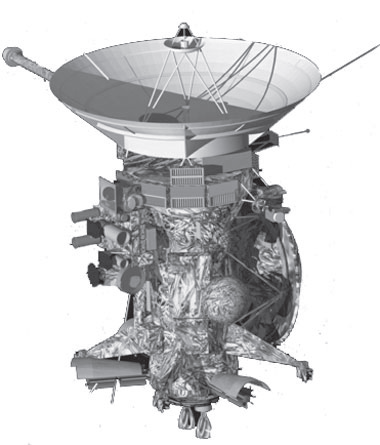
\includegraphics[width=.5\linewidth]{images/fig_00}
}%figues de la page de garde


\def\xxpied{%
%Cycle 01 -- Modéliser le comportement des systèmes multiphysiques\\
\xxactivite%
}

\setcounter{secnumdepth}{5}
%---------------------------------------------------------------------------

\usepackage{pgfplots}
\begin{document}
%\defimages{images}
%\chapterimage{png/Fond_Cin}
\pagestyle{empty}


%%%%%%%% PAGE DE GARDE COURS
\ifcours
% ==== BANDEAU DES TITRES ==== 
\begin{tikzpicture}[remember picture,overlay]
\node at (current page.north west)
{\begin{tikzpicture}[remember picture,overlay]
\node[anchor=north west,inner sep=0pt] at (0,0) {\includegraphics[width=\paperwidth]{\thechapterimage}};
\draw[anchor=west] (-2cm,-8cm) node [line width=2pt,rounded corners=15pt,draw=ocre,fill=white,fill opacity=0.6,inner sep=40pt]{\strut\makebox[22cm]{}};
\draw[anchor=west] (1cm,-8cm) node {\huge\sffamily\bfseries\color{black} %
\begin{minipage}{1cm}
\rotatebox{90}{\LARGE\sffamily\textsc{\color{ocre}\textbf{\xxnumpartie}}}
\end{minipage} \hfill
\begin{minipage}[c]{14cm}
\begin{titrepartie}
\begin{flushright}
\renewcommand{\baselinestretch}{1.1} 
\Large\sffamily\textsc{\textbf{\xxpartie}}
\renewcommand{\baselinestretch}{1} 
\end{flushright}
\end{titrepartie}
\end{minipage} \hfill
\begin{minipage}[c]{3.5cm}
{\large\sffamily\textsc{\textbf{\color{ocre} \discipline}}}
\end{minipage} 
 };
\end{tikzpicture}};
\end{tikzpicture}
% ==== FIN BANDEAU DES TITRES ==== 


% ==== ONGLET 
\begin{tikzpicture}[overlay]
\node[shape=rectangle, 
      rounded corners = .25 cm,
	  draw= ocre,
	  line width=2pt, 
	  fill = ocre!10,
	  minimum width  = 2.5cm,
	  minimum height = 3cm,] at (18.3cm,0) {};
\node at (17.7cm,0) {\rotatebox{90}{\textbf{\Large\color{ocre}{\classe}}}};
%{};
\end{tikzpicture}
% ==== FIN ONGLET 


\vspace{3.5cm}

\begin{tikzpicture}[remember picture,overlay]
\draw[anchor=west] (-2cm,-6cm) node {\huge\sffamily\bfseries\color{black} %
\begin{minipage}{2cm}
\begin{center}
\LARGE\sffamily\textsc{\color{ocre}\textbf{\xxactivite}}
\end{center}
\end{minipage} \hfill
\begin{minipage}[c]{15cm}
\begin{titrechapitre}
\renewcommand{\baselinestretch}{1.1} 
\Large\sffamily\textsc{\textbf{\xxnumchapitre}}

\Large\sffamily\textsc{\textbf{\xxchapitre}}
\vspace{.5cm}

\renewcommand{\baselinestretch}{1} 
\normalsize\normalfont
\xxcompetences
\end{titrechapitre}
\end{minipage}  };
\end{tikzpicture}
\vfill

\begin{flushright}
\begin{minipage}[c]{.3\linewidth}
\begin{center}
\xxfigures
\end{center}
\end{minipage}\hfill
\begin{minipage}[c]{.6\linewidth}
\startcontents
%\printcontents{}{1}{}
\printcontents{}{1}{}
\end{minipage}
\end{flushright}

\begin{tikzpicture}[remember picture,overlay]
\draw[anchor=west] (4.5cm,-.7cm) node {
\begin{minipage}[c]{.2\linewidth}
\begin{flushright}

\includegraphics[width=2cm]{logoCC}
\end{flushright}
\end{minipage}
\begin{minipage}[c]{.2\linewidth}
\textsl{\xxauteur} \\
\textsl{\classe}
\end{minipage}
 };
\end{tikzpicture}

\newpage
\pagestyle{fancy}

%\newpage
%\pagestyle{fancy}

\else
\fi
%% FIN PAGE DE GARDE DES COURS

%%%%%%%% PAGE DE GARDE TD
\iftd
%\begin{tikzpicture}[remember picture,overlay]
%\node at (current page.north west)
%{\begin{tikzpicture}[remember picture,overlay]
%\draw[anchor=west] (-2cm,-3.25cm) node [line width=2pt,rounded corners=15pt,draw=ocre,fill=white,fill opacity=0.6,inner sep=40pt]{\strut\makebox[22cm]{}};
%\draw[anchor=west] (1cm,-3.25cm) node {\huge\sffamily\bfseries\color{black} %
%\begin{minipage}{1cm}
%\rotatebox{90}{\LARGE\sffamily\textsc{\color{ocre}\textbf{\xxnumpartie}}}
%\end{minipage} \hfill
%\begin{minipage}[c]{13.5cm}
%\begin{titrepartie}
%\begin{flushright}
%\renewcommand{\baselinestretch}{1.1} 
%\Large\sffamily\textsc{\textbf{\xxpartie}}
%\renewcommand{\baselinestretch}{1} 
%\end{flushright}
%\end{titrepartie}
%\end{minipage} \hfill
%\begin{minipage}[c]{3.5cm}
%{\large\sffamily\textsc{\textbf{\color{ocre} \discipline}}}
%\end{minipage} 
% };
%\end{tikzpicture}};
%\end{tikzpicture}

%%%%%%%%%% PAGE DE GARDE TD %%%%%%%%%%%%%%%
%\begin{tikzpicture}[overlay]
%\node[shape=rectangle, 
%      rounded corners = .25 cm,
%	  draw= ocre,
%	  line width=2pt, 
%	  fill = ocre!10,
%	  minimum width  = 2.5cm,
%	  minimum height = 2.5cm,] at (18.5cm,0) {};
%\node at (17.7cm,0) {\rotatebox{90}{\textbf{\Large\color{ocre}{\classe}}}};
%%{};
%\end{tikzpicture}

% PARTIE ET CHAPITRE
%\begin{tikzpicture}[remember picture,overlay]
%\draw[anchor=west] (-1cm,-2.1cm) node {\large\sffamily\bfseries\color{black} %
%\begin{minipage}[c]{15cm}
%\begin{flushleft}
%\xxnumchapitre \\
%\xxchapitre
%\end{flushleft}
%\end{minipage}  };
%\end{tikzpicture}

% BANDEAU EXO
\iflivret % SI LIVRET
\begin{tikzpicture}[remember picture,overlay]
\draw[anchor=west] (-2cm,-3.3cm) node {\huge\sffamily\bfseries\color{black} %
\begin{minipage}{5cm}
\begin{center}
\LARGE\sffamily\color{ocre}\textbf{\textsc{\xxactivite}}

\begin{center}
\xxfigures
\end{center}

\end{center}
\end{minipage} \hfill
\begin{minipage}[c]{12cm}
\begin{titrechapitre}
\renewcommand{\baselinestretch}{1.1} 
\large\sffamily\textbf{\textsc{\xxtitreexo}}

\small\sffamily{\textbf{\textit{\color{black!70}\xxsourceexo}}}
\vspace{.5cm}

\renewcommand{\baselinestretch}{1} 
\normalsize\normalfont
\xxcompetences
\end{titrechapitre}
\end{minipage}};
\end{tikzpicture}
\else % ELSE NOT LIVRET
\begin{tikzpicture}[remember picture,overlay]
\draw[anchor=west] (-2cm,-4.5cm) node {\huge\sffamily\bfseries\color{black} %
\begin{minipage}{5cm}
\begin{center}
\LARGE\sffamily\color{ocre}\textbf{\textsc{\xxactivite}}

\begin{center}
\xxfigures
\end{center}

\end{center}
\end{minipage} \hfill
\begin{minipage}[c]{12cm}
\begin{titrechapitre}
\renewcommand{\baselinestretch}{1.1} 
\large\sffamily\textbf{\textsc{\xxtitreexo}}

\small\sffamily{\textbf{\textit{\color{black!70}\xxsourceexo}}}
\vspace{.5cm}

\renewcommand{\baselinestretch}{1} 
\normalsize\normalfont
\xxcompetences
\end{titrechapitre}
\end{minipage}};
\end{tikzpicture}

\fi

\else   % FIN IF TD
\fi


%%%%%%%% PAGE DE GARDE FICHE
\iffiche
\begin{tikzpicture}[remember picture,overlay]
\node at (current page.north west)
{\begin{tikzpicture}[remember picture,overlay]
\draw[anchor=west] (-2cm,-2.25cm) node [line width=2pt,rounded corners=15pt,draw=ocre,fill=white,fill opacity=0.6,inner sep=40pt]{\strut\makebox[22cm]{}};
\draw[anchor=west] (1cm,-2.25cm) node {\huge\sffamily\bfseries\color{black} %
\begin{minipage}{1cm}
\rotatebox{90}{\LARGE\sffamily\textsc{\color{ocre}\textbf{\xxnumpartie}}}
\end{minipage} \hfill
\begin{minipage}[c]{14cm}
\begin{titrepartie}
\begin{flushright}
\renewcommand{\baselinestretch}{1.1} 
\large\sffamily\textsc{\textbf{\xxpartie} \\} 

\vspace{.2cm}

\normalsize\sffamily\textsc{\textbf{\xxnumchapitre -- \xxchapitre}}
\renewcommand{\baselinestretch}{1} 
\end{flushright}
\end{titrepartie}
\end{minipage} \hfill
\begin{minipage}[c]{3.5cm}
{\large\sffamily\textsc{\textbf{\color{ocre} \discipline}}}
\end{minipage} 
 };
\end{tikzpicture}};
\end{tikzpicture}

\iflivret
\begin{tikzpicture}[overlay]
\node[shape=rectangle, 
      rounded corners = .25 cm,
	  draw= ocre,
	  line width=2pt, 
	  fill = ocre!10,
	  minimum width  = 2.5cm,
	  minimum height = 2.5cm,] at (18.5cm,1.1cm) {};
\node at (17.9cm,1.1cm) {\rotatebox{90}{\textsf{\textbf{\large\color{ocre}{\classe}}}}};
%{};
\end{tikzpicture}
\else
\begin{tikzpicture}[overlay]
\node[shape=rectangle, 
      rounded corners = .25 cm,
	  draw= ocre,
	  line width=2pt, 
	  fill = ocre!10,
	  minimum width  = 2.5cm,
%	  minimum height = 2.5cm,] at (18.5cm,1.1cm) {};
	  minimum height = 2.5cm,] at (18.6cm,0cm) {};
\node at (18cm,0cm) {\rotatebox{90}{\textsf{\textbf{\large\color{ocre}{\classe}}}}};
%{};
\end{tikzpicture}

\fi

\else
\fi



\vspace{5cm}
\pagestyle{fancy}
\thispagestyle{plain}

\def\columnseprulecolor{\color{ocre}}
\setlength{\columnseprule}{0.4pt} 

%\defimages2{images}

%\begin{multicols}{2}

\lstset{language=Python,
  inputencoding=utf8/latin1,
  breaklines=true,breaklines=true,
  basicstyle=\ttfamily\footnotesize, columns=fullflexible,
  keywordstyle=\bfseries\color{green!40!black},
  commentstyle=\itshape\color{purple!40!black},
  identifierstyle=\color{blue},
  stringstyle=\color{orange}}  
\definecolor{mygreen}{rgb}{0,0.6,0}


\lstset{
     literate=%
         {é}{{\'e}}1    
         {à}{{\`a}}1    
}




\section{Exercices}
\begin{multicols}{2}
\begin{lstlisting}
def factorielle(n) :
    """
    Donnée : un entier n >= 0
    Resultat : la factorielle de n
    """
    F=1
    i =  n
    while i > 0 :
        F = F*i
        i = i-1
    return F
\end{lstlisting}
\subparagraph{}\textit{Montrer que $F \times i ! = n!$ est un invariant de boucle.}
\ifprof
\begin{corrige}
\begin{itemize}
\item À l'entrée dans la boucle, $F=1$, $i=n$;  donc $F \times i ! = n!$.
\item On considère qu'au k\ieme tour de boucle, $F_k \times i_k ! = n!$.
\item Montrons que $F_{k+1} \times i_{k+1}! =n!$. À la fin de l'itération suivante, calculons $F_{k+1} \times i_{k+1}!  = \left(F_{k} \times i_{k} \right) \times \left(i_{k} -1 \right)!  $
$= F_{k} \times \left( i_{k}  \times \left(i_{k} -1 \right)!\right)  $
$= F_{k} \times  i_{k}! = n!  $. \textit{CQFD}
\end{itemize}
\end{corrige}
\else
\fi


\begin{lstlisting}
def racine(n):
    """
    Données : un entier n >= 0
    Résultat : la racine carrée de n (arrondie à l'entier inférieur)
    """
    c = 0
    s = 1
    while s <= n :
        c =  c + 1
        s = s + 2*c + 1
    return c
\end{lstlisting}


\subparagraph{}\textit{Montrer que $n-s$ est un variant de boucle.}
\ifprof
\begin{corrige}
\begin{itemize}
\item D'après la condition du while, la quanité $n-s$ est toujours positive.
\item $n$ ne varie pas et $c$ est croissant est positif à chaque itération; donc $n-s$ décroît à chaque itération. 
\end{itemize}
$n-s$ est donc un variant de boucle.
\end{corrige}
\else
\fi

\end{multicols}
%def racine(n):
%Data : un entier n >= 0
%Result : la racine carrée de n (arrondie à l’entier inférieur)
%c := 0
%s := 1
%while s <= n do
%c := c + 1
%s := s + 2 * c + 1
%return c
%\end{lstlisting}

\section{Introduction}

\ifprof
\else
La mission spatiale Cassini-Huygens a pour objectif l'exploration de Saturne et de ses nombreux satellites naturels (62 « lunes » identifiées en 2009). Cassini orbite depuis 2004 autour de Saturne et collecte grâce à ses différents instruments d'observation, de précieuses informations sur la planète géante, ses anneaux caractéristiques
et ses différents satellites.

Le sujet proposé aborde l'acquisition d'images par l'imageur spectral VIMS (Visible and Infrared Mapping Spectrometer) dans le domaine du visible et de l'infrarouge embarqué à bord de la sonde Cassini et la compression des données avant transmission vers la Terre pour leur exploitation.
\fi
\section{Acquisition d'images par l'imageur VIMS et compression des données}
\subsection{Présentation}
\ifprof
\else
La sonde Cassini embarque à son bord un ensemble de 12 instruments scientifiques destinés à l'étude de Saturne et son système, dont 4 instruments d'observation à distance permettant de couvrir une bande spectrale d'observation très large 
(\autoref{fig_01} et \autoref{fig_02}).

\begin{minipage}[b]{.45\linewidth}
\begin{figure}[H]
\centering
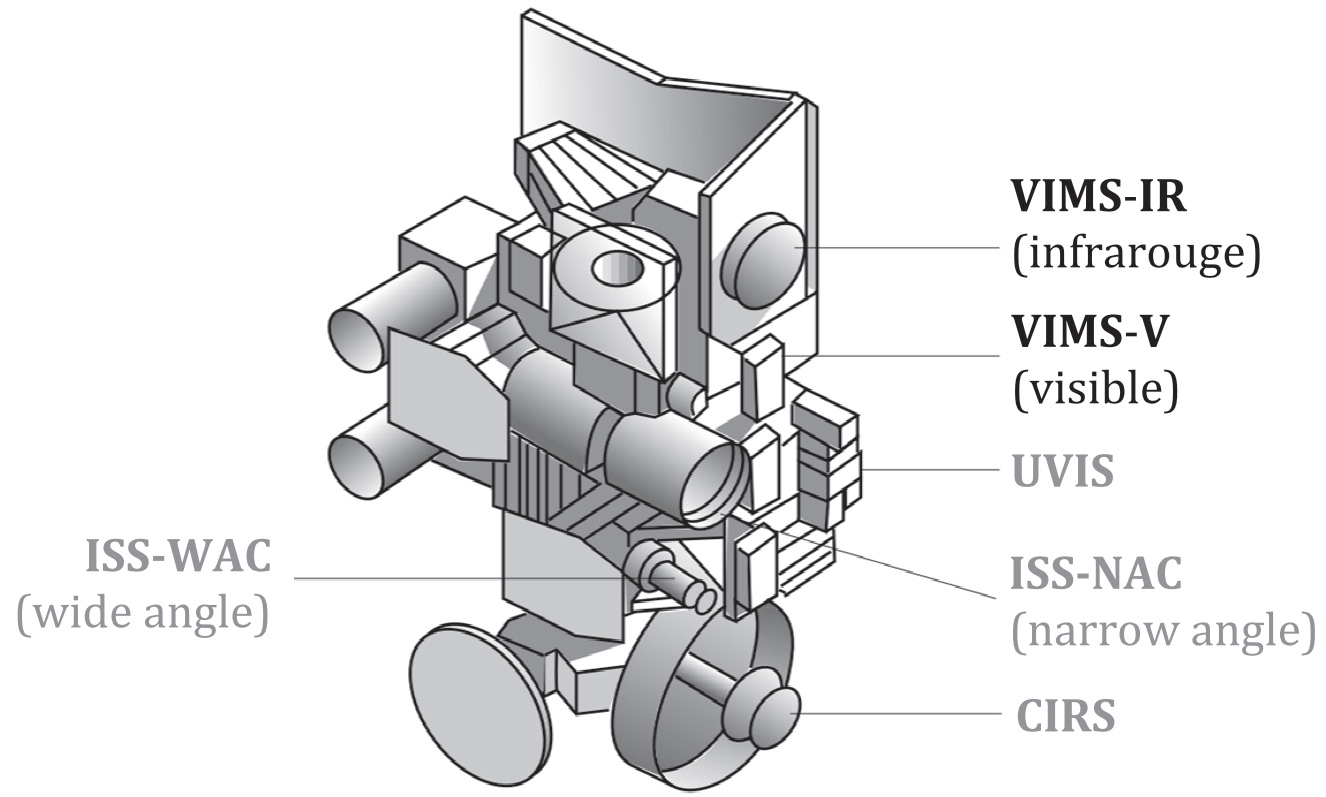
\includegraphics[width=.9\linewidth]{images/fig_01}
\caption{Instruments d'observation à distance \label{fig_01}}
\end{figure}
\end{minipage}
\hfill
\begin{minipage}[b]{.45\linewidth}
\begin{figure}[H]
\centering
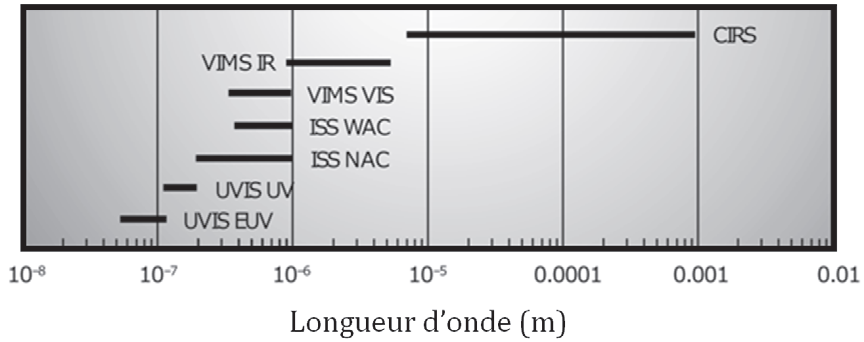
\includegraphics[width=.9\linewidth]{images/fig_02}
\caption{Domaine de travail des différents instruments d'observation à distance \label{fig_02}}
\end{figure}
\end{minipage}

\vspace{.25cm}

L'un des principaux objectifs scientifiques associés à l'instrument VIMS est de cartographier
la distribution spatiale des caractéristiques minéralogiques et chimiques de différentes cibles :
anneaux de Saturne, surface de ses satellites, atmosphère de Saturne et Titan, etc. Pour cela,
l'instrument VIMS mesure les radiations émises et réfléchies par les corps observés, sur une
gamme de 0,35 à \SI{5,1}{\mu m} (domaines visible et infrarouge) avec au total 352 longueurs d'onde
différentes.


Les données acquises par l'instrument sont organisées sous la forme d'un cube (\autoref{fig_03})
constitué d'un ensemble de 352 « tranches » (associées aux différentes longueurs d'onde $\lambda$)
comportant 64 pixels dans les deux directions spatiales $x$ et $y$. Il est ensuite possible d'en
extraire une image à une longueur d'onde donnée ($\lambda_k$) ou un spectre associé à un pixel de
coordonnées spatiales $(x_i,y_j)$.

\begin{figure}[H]
\centering
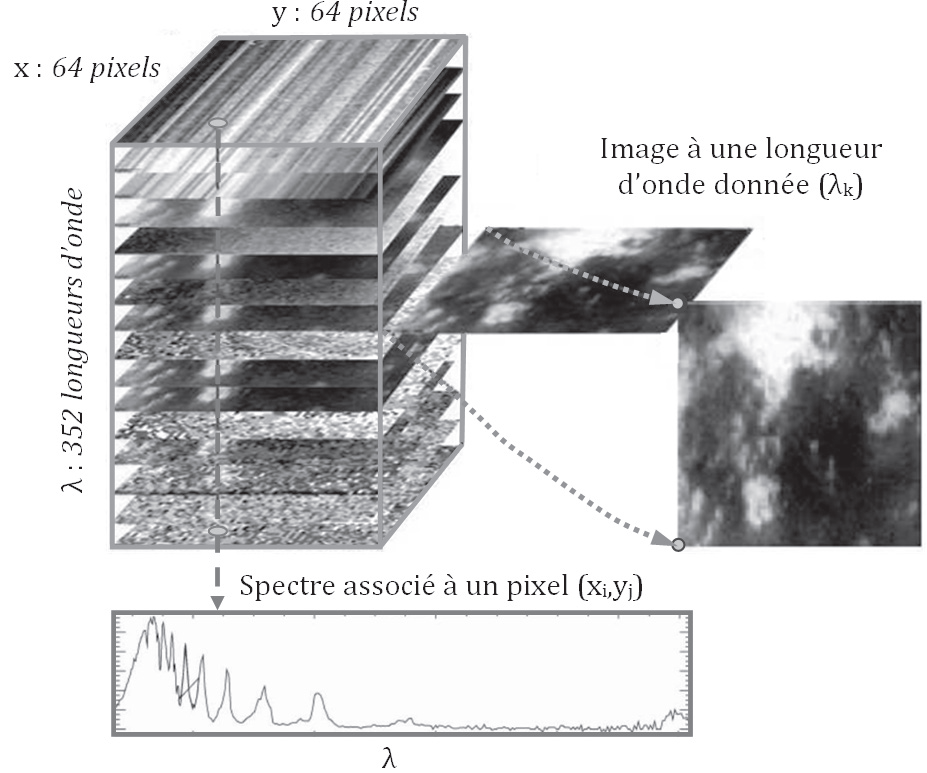
\includegraphics[width=.7\linewidth]{images/fig_03}
\caption{Structure d'un cube de données hyperspectrales \label{fig_03}}
\end{figure}



Les contraintes technologiques liées au transfert de l'ensemble des données recueillies par la
sonde vers la Terre imposent une réduction de leur volume. Pour l'imageur VIMS, cela consiste
en une compression des données prise en charge par une unité de traitement numérique embarquée
à bord de la sonde. Cette compression doit toutefois s'effectuer sans perte d'information.
Après compression, la taille maximale attendue pour un cube de données est de \SI{1}{Mo} (mégaoctet).

\begin{obj}
Cette partie s'intéresse à l'implémentation d'algorithmes spécifiques visant à améliorer
les performances de la compression en vue d'une mise à jour des programmes
de l'unité de traitement embarquée.

\textbf{Après compression, la taille maximale attendue pour un cube de données est de \SI{1}{Mo} (mégaoctet).}
\end{obj}



À chaque pixel $p_{ijk}$ du cube de données hyperspectrales (de coordonnées $x_i$, $y_j$ et appartenant
à une image de longueur d'onde $\lambda_k$) est associé un nombre moyen de photons reçus par les
capteurs de l'instrument VIMS. Cette dernière information est codée sur 12 bits.


On rappelle qu'un octet est égal à 8 bits.
\fi


\subparagraph{}\textit{Déterminer en octets la taille d'un cube de données hyperspectrales avant compression.}
\ifprof
\begin{corrige} La taille d'une image est de $t_i = 64 \times 64 \times 12= \SI{49152}{bits} $ soit, pour le cube une taille de $t_c = t_i\times 352 = \SI{17301504}{bits}=\SI{2 162 688}{octets}=\SI{2,16}{Mo}$.
\end{corrige}
\else
\fi


\ifprof
\else

Si $T$ et $T_c$ représentent respectivement la taille des données avant compression et après
compression, le taux de compression $\tau$ est défini comme : $\tau = \dfrac{T-T_c}{T}$.
\fi

\subparagraph{}\textit{Déterminer alors le taux de compression à appliquer aux données afin de respecter le cahier
des charges.}
\ifprof
\begin{corrige} La taux de compression à appliquer est donc $\tau = \dfrac{T-T_c}{T}= \dfrac{2,16-1}{2,16}=\SI{54}{\%}$.
\end{corrige}

\else
\fi

\subsection{Principe de la compression des données}

\ifprof
\else

La compression des données est réalisée à l'issue de l'acquisition d'une ligne (soit 64 pixels
pour la dimension spatiale et 352 longueurs d'onde pour la dimension spectrale) par l'imageur
VIMS. Les données sont traitées par blocs de 64 pixels $\times$ 32 longueurs d'onde. L'algorithme
mis en \oe{}uvre pour la compression est un algorithme dit entropique, qui réalise un codage des
données exploitant la redondance de l'information. L'exemple proposé ci-après permet d'en
illustrer le principe, avec le codage d'une suite de 10 entiers naturels.

Soit la série $S_n$ de 10 entiers naturels $s_k \in[0, 8]$ : 4 -- 5 -- 7 -- 0 -- 7 -- 8 -- 4 -- 1 -- 7 -- 4.
Un codage en binaire naturel des entiers 0 à 8 nécessitant au minimum 4 bits, le choix d'un tel
codage pour la série $S_n$ conduirait à un code d'une longueur totale de 40 bits.

La longueur du code associé à la série $S_n$ peut être réduite en adoptant un codage exploitant
les propriétés suivantes de la série :
\begin{itemize}
\item seules 6 valeurs $v_i$ sont utilisées parmi les 9 possibles;
\item certaines valeurs $v_i$ possèdent des probabilités $p_i$ d'apparition plus importantes que d'autres.
\end{itemize}

Une solution consiste par exemple à adopter un codage à longueur variable, où les codes les plus
courts sont associés aux valeurs qui possèdent la probabilité d'apparition la plus importante.

Un tel codage est proposé dans le \autoref{tab_01} pour les entiers de la série $S_n$. La série $S_n$ est
alors codée de la manière suivante.

\begin{center}
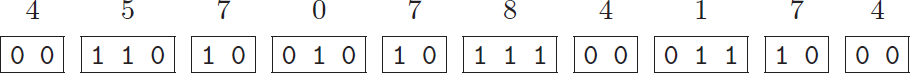
\includegraphics[width=.7\linewidth]{images/fig_04}
\end{center}



\begin{minipage}[b]{.55\linewidth}
La longueur du code associé à la série est à présent de
24 bits (soit une longueur moyenne de 2,4 bits par caractère).
Le décodage est unique, mais il nécessite la connaissance de la
table de codage établissant la correspondance entre un code
et la valeur associée.

C'est cette stratégie qui est adoptée pour les opérations
de compression. Pour la série $S_n$ considérée, avec des valeurs
initialement codées sur 4 bits en binaire naturel, le codage à
longueur variable présenté permet d'obtenir un taux de compression
$\tau = \SI{40}{\%}$.
\end{minipage}
\hfill
\begin{minipage}[b]{.4\linewidth}
\begin{table}[H]
\centering
\begin{tabular}{|c|c|c|}
\hline
Valeur $v_i$ & Probabilité $p_i$ & code \\
\hline
4 & 0,3 & \texttt{0 0}\\
7 & 0,3 & \texttt{1 0}\\
0 & 0,1 & \texttt{0 1 0}\\
1 & 0,1 & \texttt{0 1 1}\\
5 & 0,1 & \texttt{1 1 0}\\
8 & 0,1 & \texttt{1 1 1}\\
\hline
\end{tabular}
\caption{Table de codage\label{tab_01}}
\end{table}
\end{minipage}
\fi

\subsection{Limite du taux de compression}

\ifprof
\else

Les algorithmes de compression entropiques étant basés sur l'exploitation de la redondance
dans les données à coder, leur efficacité est directement liée à la « quantité d'information »
qu'elles contiennent : plus il y a répétitions de certaines valeurs dans les données à coder
(l'entropie des données est alors faible), plus le taux de compression atteint est élevé.

Une valeur limite du taux de compression que l'on peut espérer atteindre peut être approchée
par le calcul de l'entropie de Shannon $H$, grandeur fournissant une mesure de la « quantité
d'information » contenue dans les données, en bits par caractère. Pour une série de données $S_n$
(considérée comme une variable aléatoire) l'entropie $H$ est définie de la manière suivante :
$$
H\left(S_n\right)=-\sum\limits_{i=1}^{i=N_v} p_i \log_2 p_i
$$

avec :
\begin{itemize}
\item $N_v$ : nombre de valeurs $v_i$ différentes contenues dans la série ;
\item $p_i$ : probabilité d'apparition de la valeur $v_i$ ($p_i = \dfrac{n_i}{n}$ avec $n_i$ nombre d'occurrences de la valeur $v_i$ et $n$ nombre de termes de la série $S_n$) ;
\item $\log_2$ : fonction logarithme binaire (base 2). Pour $x\in \mathbb{R}$, $\log_2(x) = \dfrac{\ln(x)}{\ln(2)}$ où $\ln$ est la fonction logarithme népérien. On suppose que la fonction $\log_2(x)$ est définie dans le langage de
programmation choisi.
\end{itemize}

\fi
\subparagraph{}\textit{Calculer l'entropie associée à l'exemple précédent. En déduire le taux de compression limite
de cet exemple et le comparer à la longueur moyenne de 2,4 bits par caractère.}
\ifprof
\begin{corrige}
$H\left(S_n\right)=-\sum\limits_{i=1}^{i=6} p_i \log_2 p_i
=-2\times 0,3\log_2 0,3- 4\times 0,1\log_2 0,1=2,37$.

*****

\end{corrige}
\else
\fi


\ifprof
\else

\vspace{.5cm}

Dans le cadre d'une étude visant à améliorer les performances de la compression des données,
les ingénieurs souhaitent caractériser l'entropie des images acquises par l'instrument VIMS.
La fonction \texttt{entropie(S)} dont le code est partiellement présenté ci-après reçoit en argument
d'entrée une série d'entiers naturels $S$ sous forme de tableau à une dimension (liste en Python)
et renvoie la valeur $H$ de l'entropie de Shannon associée.

\begin{lstlisting}
def entropie (S) :
    # 1. Commentaire question 4
    valeurs = list(set(S))
    # 2. Détermination du nombre d'occurrences (nombre d'apparitions) 
    # occ_i de chaque valeur v_i et calcul de la probabilité proba[i] associée.
    # QUESTION Q5 : zone à compléter
    # 3. Calcul de l'entropie de Shannon H
    # QUESTION Q6 : zone à compléter
    return H
\end{lstlisting}

La fonction réalise différentes étapes. La première étape utilise la fonction \texttt{set} en Python. Un exemple extrait de la documentation de la fonction \texttt{set} est donnée
ci-dessous. En Python, il faut transformer le résultat en \texttt{list} pour itérer sur le résultat de \texttt{set}.

\begin{lstlisting}
>>> basket = ['apple', 'orange', 'apple', 'pear', 'orange', 'banana']
>>> fruit = set(basket) # create a set without duplicates
>>> fruit
    set (['orange', 'pear', 'apple', 'banana'])
>>> 'orange' in fruit # fast membership testing
    True
>>>'crabgrass' in fruit
    False
\end{lstlisting}

\fi

\subparagraph{}\textit{Compléter le commentaire 1 de la fonction \texttt{entropie(S)} correspondant à la ligne de programme définissant la variable \texttt{valeurs}.}
\ifprof
\begin{corrige}
\end{corrige}
\else
\fi


\subparagraph{}\textit{Compléter la 2\ieme étape de la fonction \texttt{entropie(S)} à partir du commentaire afin de calculer les probabilités $p_i$.}
\ifprof
\begin{corrige}
\end{corrige}
\else
\fi


\subparagraph{}\textit{Compléter la 3\ieme étape de la fonction \texttt{entropie(S)} afin de calculer l’entropie de Shannon
$H$ définie par l’équation (1).}
\ifprof
\begin{corrige}
Questions 4, 5 et 6.

\begin{lstlisting}
def entropie (S) :
    # Question 4
    """ Détermine l'entropie à partir d'une liste d'entiers :
     * S (list[int])
     * H : entropie
    """ 
    valeurs = list(set(S))
    # Question 5
    prob = []
    for v in valeurs :
        nb_occ = 0
        	for el in S : 
        	    if el == v :
        	        nb_occ=nb_occ+1
        prob.append(nb_occ/len(S))

    # Question 6        
    H = 0
    for p in prob : 
        H=H-p*log2(p)
   
    return H
\end{lstlisting}
\end{corrige}
\else
\fi

Suite à une acquisition d’image par l’instrument VIMS, l’utilisateur dispose de données
brutes dont il souhaite évaluer l’entropie. Un bloc élémentaire de données se présente sous la
forme d’un tableau à une dimension \texttt{bloc\_image} constitué de valeurs entières (allant de 0 à
$4 095 = 2^{12} - 1$).

On rappelle que $H$ est une valeur limite du taux de compression que l'on peut espérer atteindre.

\subparagraph{}\textit{Écrire la suite d’instructions permettant de calculer et d’afficher la valeur du taux de
compression limite $\tau$ associé aux données contenues dans le tableau \texttt{bloc\_image}.}
\ifprof
\begin{corrige}~\\
\begin{lstlisting}
n = 4095
H = entropie(bloc_image)
tau=(n*12-n*H)/(n*12)
\end{lstlisting}
\end{corrige}
\else
\fi

\subsection{Prétraitement des données avant compression}

\ifprof
\else

Les données brutes sont traitées par blocs correspondants à une acquisition de 64 pixels
(dimension spatiale $y$) par 32 longueurs d’onde (dimension spectrale $\lambda$). Ces données sont
organisées sous forme d’une matrice \texttt{donnees\_brutes} composée de 32 lignes et 64 colonnes.


Une stratégie efficace permettant d’améliorer la compression consiste à réaliser un prétraitement
des données visant à réduire leur entropie. Il a été constaté pour les images acquises par
l’instrument VIMS que les importantes variations de luminance (intensité lumineuse par unité
de surface) constituent la contribution dominante dans l’entropie des données. Ainsi, le prétraitement
consiste à estimer ces variations, puis à les soustraire aux données brutes à compresser
afin de constituer un nouvel ensemble de données, d’entropie inférieure.

La procédure de prétraitement consiste d’abord à construire une matrice modèle
\texttt{matrice\_modele} permettant d’estimer les variations de luminance associées au bloc de données
brutes. 

\textit{Pour information, les étapes sont décrites ci-après :
\begin{enumerate}
\item construction d’une ligne \texttt{luminance\_moy} représentative de la luminance moyenne, en
effectuant la moyenne de 4 lignes de la matrice \texttt{donnees\_brutes} régulièrement espacées
et associées à différentes longueurs d’ondes $\lambda_i$, $i = 1, 11, 21, 31$ ;
\item identification du pixel de luminance maximale (de valeur \texttt{luminance\_max}) dans la ligne
moyenne \texttt{luminance\_moy} construite à l’étape précédente ;
\item extraction d’un vecteur colonne \texttt{spectre\_max} contenant le spectre (32 composantes)
associé au pixel de luminance maximale ;
\item normalisation du vecteur \texttt{spectre\_max} en divisant (division réelle) chacune de ses composantes
par la valeur \texttt{luminance\_max} relevée à l’étape 2. Le résultat est une liste contenant
des réels ;
\item construction de la matrice modèle \texttt{matrice\_modele} de dimension (32 lignes, 64 colonnes)
en effectuant le produit du vecteur colonne \texttt{spectre\_max} par la ligne de luminance
moyenne \texttt{luminance\_moy}.
\end{enumerate}}
%
%
%
%
%\subparagraph{}\textit{À partir de la description des étapes 1 et 2, écrire une fonction \texttt{pretraitement12(donnees\_
%brutes)} recevant en argument d’entrée la matrice \texttt{donnees\_brutes} et renvoyant le vecteur
%ligne \texttt{luminance\_moy}, la valeur de luminance maximale \texttt{luminance\_max} relevée pour cette
%ligne moyenne, ainsi que l’indice $j$ (variable \texttt{j\_max}) associé (sans utiliser la fonction max interne
%au langage).}
%\ifprof
%\begin{corrige}
%
%\begin{lstlisting}
%
%def pretraitement12(donnees_brutes):
%    luminance_moy=[]
%    for i in range(64):
%        somme=0
%        for indice in [0,10,20,30]:
%            somme+=donnees_brutes[indice][i]
%        luminance_moy.append(somme/4)
%    j_max=0
%    luminance_max=luminance_moy[0]
%    for j in range(64):
%        if luminance_moy[j]>luminance_max:
%            luminance_max=luminance_moy[j]
%            j_max=j
%    return(array([luminance_moy]),luminance_max,j_max)
%\end{lstlisting}
%\end{corrige}
%\else
%\fi
%
%\subparagraph{}\textit{À partir de la description des étapes 3 et 4, écrire une fonction \texttt{pretraitement34(donnees\_
%brutes, luminance\_max,j\_max)} recevant en argument d’entrée la matrice \texttt{donnees\_brutes},
%la valeur de luminance maximale \texttt{luminance\_max} ainsi que l’indice \texttt{j\_max} et renvoyant le vecteur
%colonne \texttt{spectre\_max} normalisé.}
%\ifprof
%\begin{corrige}
%
%\begin{lstlisting}
%
%def pretraitement34(donnees_brutes,luminance_max,j_max):
%    spectre_max=ones((32,1))
%    for i in range(32):
%        spectre_max[i][0]=donnees_brutes[i][j_max]
%    spectre_max=spectre_max/luminance_max
%    return spectre_max
%\end{lstlisting}
%\end{corrige}
%\else
%\fi
%
%\subparagraph{}\textit{À partir de la description de l’étape 5, écrire une fonction \texttt{pretraitement5(luminance\_
%moy, spectre\_max)} recevant en argument d’entrée le vecteur ligne \texttt{luminance\_moy}, le vecteur
%colonne \texttt{spectre\_max} et renvoyant la matrice modèle \texttt{matrice\_modele}.
%La matrice modèle \texttt{matrice\_modele} obtenue constitue une estimation des variations de
%luminance associées au bloc de données brutes. Elle est alors soustraite à la matrice \texttt{donnees\_
%brutes} pour construire la matrice de données prétraitées \texttt{matrice\_pretraitee}.}
%\ifprof
%\begin{corrige}
%
%\begin{lstlisting}
%
%def pretraitement5(luminance_moy,spectre_max):
%    matrice_modele=ones((32,64))
%    for i in range(32):
%        for j in range(64):
%            matrice_modele[i][j]=luminance_moy[0][j]*spectre_max[i][0]
%    return matrice_modele
%\end{lstlisting}
%\end{corrige}
%\else
%\fi
%
%
%%\subparagraph{}\textit{Évaluer la complexité calculatoire (additions, soustractions, ...) associée à chacune des
%%fonctions de prétraitement, en fonction des dimensions de la matrice modèle (n lignes, m colonnes).
%%En déduire la complexité calculatoire de la phase de prétraitement.
%%}
%%\ifprof
%%\begin{corrige}
%%\end{corrige}
%%\else
%%\fi


\fi
\subsection{Compression des données}

\ifprof
\else


Les données de la matrice \texttt{matrice\_pretraitee}, d’entropie réduite, sont ensuite envoyées
vers le compresseur qui prend en charge leur compression. Il en est de même pour les vecteurs 
\texttt{luminance\_moy} et \texttt{spectre\_max} qui sont nécessaires à la reconstruction des données après
réception. L’architecture fonctionnelle du compresseur qui prend en charge ces opérations est
décrite sur la \autoref{fig_05}.

\begin{figure}[H]
\centering
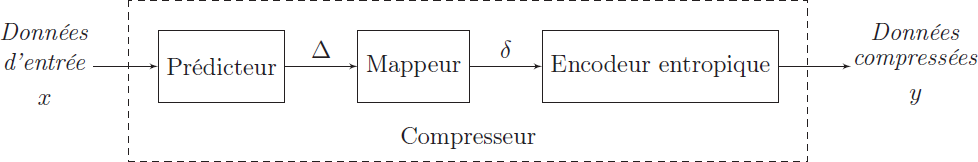
\includegraphics[width=.7\linewidth]{images/fig_05}
\caption{Architecture fonctionnelle du compresseur \label{fig_05}}
\end{figure}


Le compresseur est composé :
\begin{itemize}
\item d’un prédicteur, qui effectue une prédiction $\hat{x}_k$ pour chaque échantillon ${x}_k$ des données
d’entrée x. La prédiction $\hat{x}_k$ est réalisée simplement ici, en prenant la valeur ${x}_{k-1}$ de
l’échantillon précédent. Le prédicteur retourne l’erreur $\Delta_k$, différence entre la valeur de
l’échantillon ${x}_k$ et la prédiction $\hat{x}_k$;
\item d’un mappeur, qui réalise un mappage (correspondance) entre l’erreur de prédiction $\Delta_k$ et
un entier non signé $\delta_k$ représenté avec un nombre de bits équivalent à celui de l’échantillon
$x_k$ ;
\item d’un encodeur entropique, qui réalise un codage sans perte des valeurs $\delta_k$ en exploitant la
redondance des données tel que présenté précédemment.
\end{itemize}
\fi

\subsubsection{Prédiction du mappage}

\ifprof
\else


\begin{minipage}[c]{.55\linewidth}
Le sous-ensemble prédicteur-mappeur a pour fonction
d’associer aux échantillons d’entrée $x_k$ une série
d’entiers $\delta_k$. Cette association est réalisée de telle sorte
que les valeurs $\delta_k$ les plus faibles (donc celles qui pourront
être codées avec le moins de bits) sont celles qui
ont la probabilité d’apparition la plus élevée.

Pour l’application proposée ici, le compresseur reçoit
en entrée les données $x$ constituées d’un paquet de 32
échantillons $x_k$. Les échantillons $x_k$ considérés étant des
entiers naturels représentés sur 12 bits, les valeurs associées
appartiennent à l’intervalle $I = [0 , 4 095 = 2^{12}-1]$.
\end{minipage}
\hfill
\begin{minipage}[c]{.4\linewidth}
\begin{table}[H]
\centering
\begin{tabular}{|c|c|c|c|c|c|}
\hline
$k$ & $x_k$ & $\hat{x}_k$ & $\Delta_k$ & $\theta_k$ & $\delta_k$  \\
\hline
1 & 2 025 & -- & --  & --  & --  \\ \hline
2 & 2 027 & 2 025 & 2 & 2 025 & 4 \\ \hline
3 & 2 032 & 2 027 & 5 & 2 027 & 10 \\ \hline
4 & 2 041 & 2 032 & 9 & 2 032 & 18 \\ \hline
5 & 2 050 & 2 041 & 9 & 2 041 & 18 \\ \hline
6 & 2 053 & 2 050 & 3 & 2 045 & 6 \\ \hline
7 & 2 052 & 2 053 & $-1$ & 2 042 & 1 \\ \hline
8 & 2 050 & 2 052 & $-2$ & 2 043 & 3 \\ \hline
\vdots & \vdots& \vdots&\vdots &\vdots & \vdots\\
\hline
\end{tabular}
\caption{Illustration de la prédiction et du mappage de l’erreur associée\label{tab_02}}
\end{table}
\end{minipage}


\vspace{.25cm}

Le tableau 2 illustre les opérations réalisées par le prédicteur et le mappeur permettant d’obtenir la série
de valeur $\delta_k$:
\begin{itemize}
\item le premier échantillon $x_1 = 2 025$ est un échantillon de référence sur lequel se base la prédiction au rang
suivant $\hat{x}_2$;
\item à partir du deuxième échantillon, l’erreur de prédiction $\Delta_k = x_k - \hat{x}_k$ est calculée ;
\item un entier non signé $\delta_k$ est associé à l’erreur de prédiction $\Delta_k$ par la fonction de mappage
définie comme :
$$
\delta_k = \left\{
\begin{array}{llr}
2\Delta_k & \text{si } 0\leq \Delta_k \leq \theta_k & \\
2\left|\Delta_k \right| - 1& \text{si } -\theta_k \leq \Delta_k <0 & (2)\\
\theta_k + \left|\Delta_k \right|  & \text{sinon } & \\
\end{array}
\right.
$$
avec $\theta_k= \min\left( \hat{x}_k - x_{\text{min}}, x_{\text{max}} -\hat{x}_k \right)$, soit ici :
$\theta_k=\min \left( \hat{x}_k, 4095 - \hat{x}_k\right)$.
\end{itemize}
\fi




\subparagraph{}\textit{Écrire une fonction \texttt{prediction(x)} recevant en argument d’entrée le tableau à une dimension \texttt{x} et renvoyant le tableau \texttt{erreur} contenant les valeurs $\Delta_k$.}
\ifprof
\begin{corrige}

\begin{lstlisting}

def prediction(x):
    return [x[i]-x[i-1] for i in range(1,len(x))]# on pourrait mettre 32 à la place de len(x)
\end{lstlisting}
\end{corrige}
\else
\fi

\subparagraph{}\textit{À partir de la définition de la fonction de mappage, équation (2), écrire une fonction
\texttt{mappage(erreur,x)} recevant en arguments d’entrée les tableaux à une dimension \texttt{erreur} et \texttt{x}
et renvoyant le tableau \texttt{delta} contenant les valeurs $\delta_k$.}
\ifprof
\begin{corrige}
\begin{lstlisting}

def mappage(erreur,x):
    delta=[]
    for i in range(1,len(x)):
        theta=min([x[i-1],4095-x[i-1]])
        if erreur[i-1]<=theta and erreur[i-1]>=0:
            delta.append(2*erreur[i-1])
        elif erreur[i-1]<0 and erreur[i-1]>=-theta:
            delta.append(-2*erreur[i-1]-1)
        else:
            delta.append(theta-erreur[i-1])
    return delta
\end{lstlisting}
\end{corrige}
\else
\fi


\subsubsection{Codage entropique - Algorithme de Rice}

\ifprof
\else

L’ensemble de valeurs $\delta_k$ est ensuite codé en utilisant un codage entropique spécifique : le codage
de Rice. Celui-ci est particulièrement adapté à la compression de données dans lesquelles
les valeurs les plus faibles sont celles qui ont la probabilité d’apparition la plus élevée, mais
également lorsque la vitesse d’exécution de l’algorithme est un paramètre important.


Le principe du codage d’un entier $N$ avec l’algorithme de Rice de paramètre $p$ est le suivant :
\begin{itemize}
\item l’entier $N$ à coder est divisé par $2^p$ (division entière) ;
\item le quotient $q$ de la division entière est codé avec un codage unaire ($q$ occurrences de 1
suivies d’un 0, voir \autoref{tab_03}), ce qui constitue la première partie du code de Rice ;
\item le reste $r$ de la division entière est codé en binaire sur $p$ bits, ce qui constitue la seconde
partie du code de Rice.
\end{itemize}
Le \autoref{tab_04} illustre le codage des entiers 0 à 7 avec un codage de Rice de paramètre $p = 2$.
Une procédure d’analyse de l’ensemble de valeurs $\delta_k$ à coder permet de déterminer la valeur
optimale $p_{opt}$ du paramètre $p$. Le codage de chaque valeur $\delta_k$ est ensuite réalisé par une fonction
\texttt{codage(delta\_k,p\_opt)} recevant en argument d’entrée la valeur $\delta_k$ et l’entier $p_{\text{opt}}$ et renvoyant
le code de Rice associé.


\begin{minipage}[b]{.45\linewidth}
\begin{table}[H]
\centering
\begin{tabular}{|c|c|}
\hline
Décimal & Code unaire \\
\hline
0& 0 \\
1& 10 \\
2& 110 \\
3& 1110 \\
4& 11110 \\
5& 111110 \\
6& 1111110 \\
7& 11111110 \\ \hline
\end{tabular}
\caption{Codage unaire des entiers 0 à 7 \label{tab_03}}
\end{table}
\end{minipage}
\hfill
\begin{minipage}[b]{.45\linewidth}
\begin{table}[H]
\centering
\begin{tabular}{|c|c|}
\hline
Décimal & Rice $p=2$\\
\hline
0 & 0 00 \\
1 & 0 01 \\
2 & 0 10 \\
3 & 0 11 \\
4 & 10 00 \\
5 & 10 01 \\
6 & 10 10 \\
7 & 10 11 \\
\hline
\end{tabular}
\caption{Codage de Rice de paramètre $p = 2$ des entiers 0 à 7 \label{tab_04}}
\end{table}
\end{minipage}

\vspace{.25cm}
\fi

\subparagraph{}\textit{Déterminer le code de Rice associé à la suite de valeurs $\delta_k$ données dans le \autoref{tab_02},
page 7 pour $p = 3$. On pourra remplir le tableau suivant.}


\ifprof
\else

\begin{center}
\begin{tabular}{|p{0.1\textwidth}|p{0.1\textwidth}|p{0.1\textwidth}|p{0.1\textwidth}|p{0.1\textwidth}|p{0.1\textwidth}|}
\hline
$\delta_k$& Quotien par $2^p=8$ & Codage unaire & Reste & Codage binaire & Codage Complet \\
\hline 
4 &  &  &  &  &  \\ 
\hline 
10 &  &  &  &  &  \\ 
\hline 
18 &  &  &  &  &  \\ 
\hline 
18 &  &  &  &  &  \\ 
\hline 
6 &  &  &  &  &  \\ 
\hline 
1 &  &  &  &  &  \\ 
\hline 
3 &  &  &  &  &  \\ 
\hline 
\end{tabular}
\end{center}

\fi

\ifprof
\begin{corrige} ~\\
\begin{center}
\begin{tabular}{|p{0.1\textwidth}|p{0.1\textwidth}|p{0.1\textwidth}|p{0.1\textwidth}|p{0.1\textwidth}|p{0.1\textwidth}|}
\hline
$\delta_k$& Quotient par $2^p=8$ & Codage unaire & Reste & Codage binaire & Codage Complet \\
\hline
4 & 0 & 0 & 4 & 100 & 0-100\\
\hline
10 & 1 & 10 & 2 & 010 & 10-010\\
\hline
18 & 2 & 110 & 2 & 010 & 110-010\\
\hline
18 & 2 & 110 & 2 & 010 & 110-010\\
\hline
6 & 0 & 0 & 6 & 110 & 0-110\\
\hline
1 & 0 & 0 & 1 & 001 & 0-001\\
\hline
3 & 0 & 0 & 3 & 011 & 0-011\\
\hline
\end{tabular}
\end{center}


\end{corrige}
\else
\fi

\subparagraph{}\textit{Définir la suite d’instructions de la fonction \texttt{codage(delta\_k,p\_opt)} permettant d’obtenir
un tableau à une ligne code1 associé à la première partie du code de Rice (codage unaire
du quotient).}
\ifprof
\begin{corrige}
\end{corrige}
\else
\fi

\subparagraph{}\textit{Définir la suite d’instructions de la fonction  \texttt{codage(delta\_k,p\_opt)} permettant d’obtenir
un tableau à une ligne \texttt{code2} associé à la seconde partie du code de Rice (codage binaire
du reste) et réalisant ensuite l’assemblage des deux parties dans le tableau code. L'instruction
\texttt{bin} de Python pourra être utilisée. Elle permet de convertir nu entier en binaire (on
supposera que cette fonction renvoie une chaîne de caractères associée au code binaire).}
\ifprof
\begin{corrige}

\begin{lstlisting}
def codage(delta_k,p_opt):#résultat sous forme d'un tableau
    #Q15    
    quotient=delta_k//2**p_opt
    code1=[1 for i in range(quotient)]
    code1+=[0]
    #Q16
    reste=delta_k%2**p_opt#codable sur p_opt bits
    code2=[int(i) for i in bin(reste)[2:]]
    for i in range(p_opt-len(code2)):
        code2=[0]+code2
    code=code1+code2
    return code
\end{lstlisting}
\end{corrige}
\else
\fi


\ifprof
\else
\vfill
\begin{center}
\textbf{	Fin du sujet	}
\end{center}
\vfill
\fi

\end{document}
